\documentclass[11pt,a4paper]{report}
\usepackage[textwidth=37em,vmargin=30mm]{geometry}
\usepackage{calc,xunicode,amsmath,amssymb,paralist,enumitem,tabu,booktabs,datetime2,xeCJK,xeCJKfntef,listings}
\usepackage{tocloft,fancyhdr,tcolorbox,xcolor,graphicx,eso-pic,xltxtra,xelatexemoji}

\newcommand{\envyear}[0]{2025}
\newcommand{\envdatestr}[0]{2025-07-02}
\newcommand{\envfinaldir}[0]{webdb/2025/20250702/final}

\usepackage[hidelinks]{hyperref}
\hypersetup{
    colorlinks=false,
    pdfpagemode=FullScreen,
    pdftitle={Web Digest - \envdatestr}
}

\setlength{\cftbeforechapskip}{10pt}
\renewcommand{\cftchapfont}{\rmfamily\bfseries\large\raggedright}
\setlength{\cftbeforesecskip}{2pt}
\renewcommand{\cftsecfont}{\sffamily\small\raggedright}

\setdefaultleftmargin{2em}{2em}{1em}{1em}{1em}{1em}

\usepackage{xeCJK,xeCJKfntef}
\xeCJKsetup{PunctStyle=plain,RubberPunctSkip=false,CJKglue=\strut\hskip 0pt plus 0.1em minus 0.05em,CJKecglue=\strut\hskip 0.22em plus 0.2em}
\XeTeXlinebreaklocale "zh"
\XeTeXlinebreakskip = 0pt


\setmainfont{Brygada 1918}
\setromanfont{Brygada 1918}
\setsansfont{IBM Plex Sans}
\setmonofont{JetBrains Mono NL}
\setCJKmainfont{Noto Serif CJK SC}
\setCJKromanfont{Noto Serif CJK SC}
\setCJKsansfont{Noto Sans CJK SC}
\setCJKmonofont{Noto Sans CJK SC}

\setlength{\parindent}{0pt}
\setlength{\parskip}{8pt}
\linespread{1.15}

\lstset{
	basicstyle=\ttfamily\footnotesize,
	numbersep=5pt,
	backgroundcolor=\color{black!5},
	showspaces=false,
	showstringspaces=false,
	showtabs=false,
	tabsize=2,
	captionpos=b,
	breaklines=true,
	breakatwhitespace=true,
	breakautoindent=true,
	linewidth=\textwidth
}






\newcommand{\coverpic}[2]{
    % argv: itemurl, authorname
    Cover photo by #2~~(\href{#1}{#1})
}
\newcommand{\makeheader}[0]{
    \begin{titlepage}
        % \newgeometry{hmargin=15mm,tmargin=21mm,bmargin=12mm}
        \begin{center}
            
            \rmfamily\scshape
            \fontspec{BaskervilleF}
            \fontspec{Old Standard}
            \fontsize{59pt}{70pt}\selectfont
            WEB\hfill DIGEST
            
            \vfill
            % \vskip 30pt
            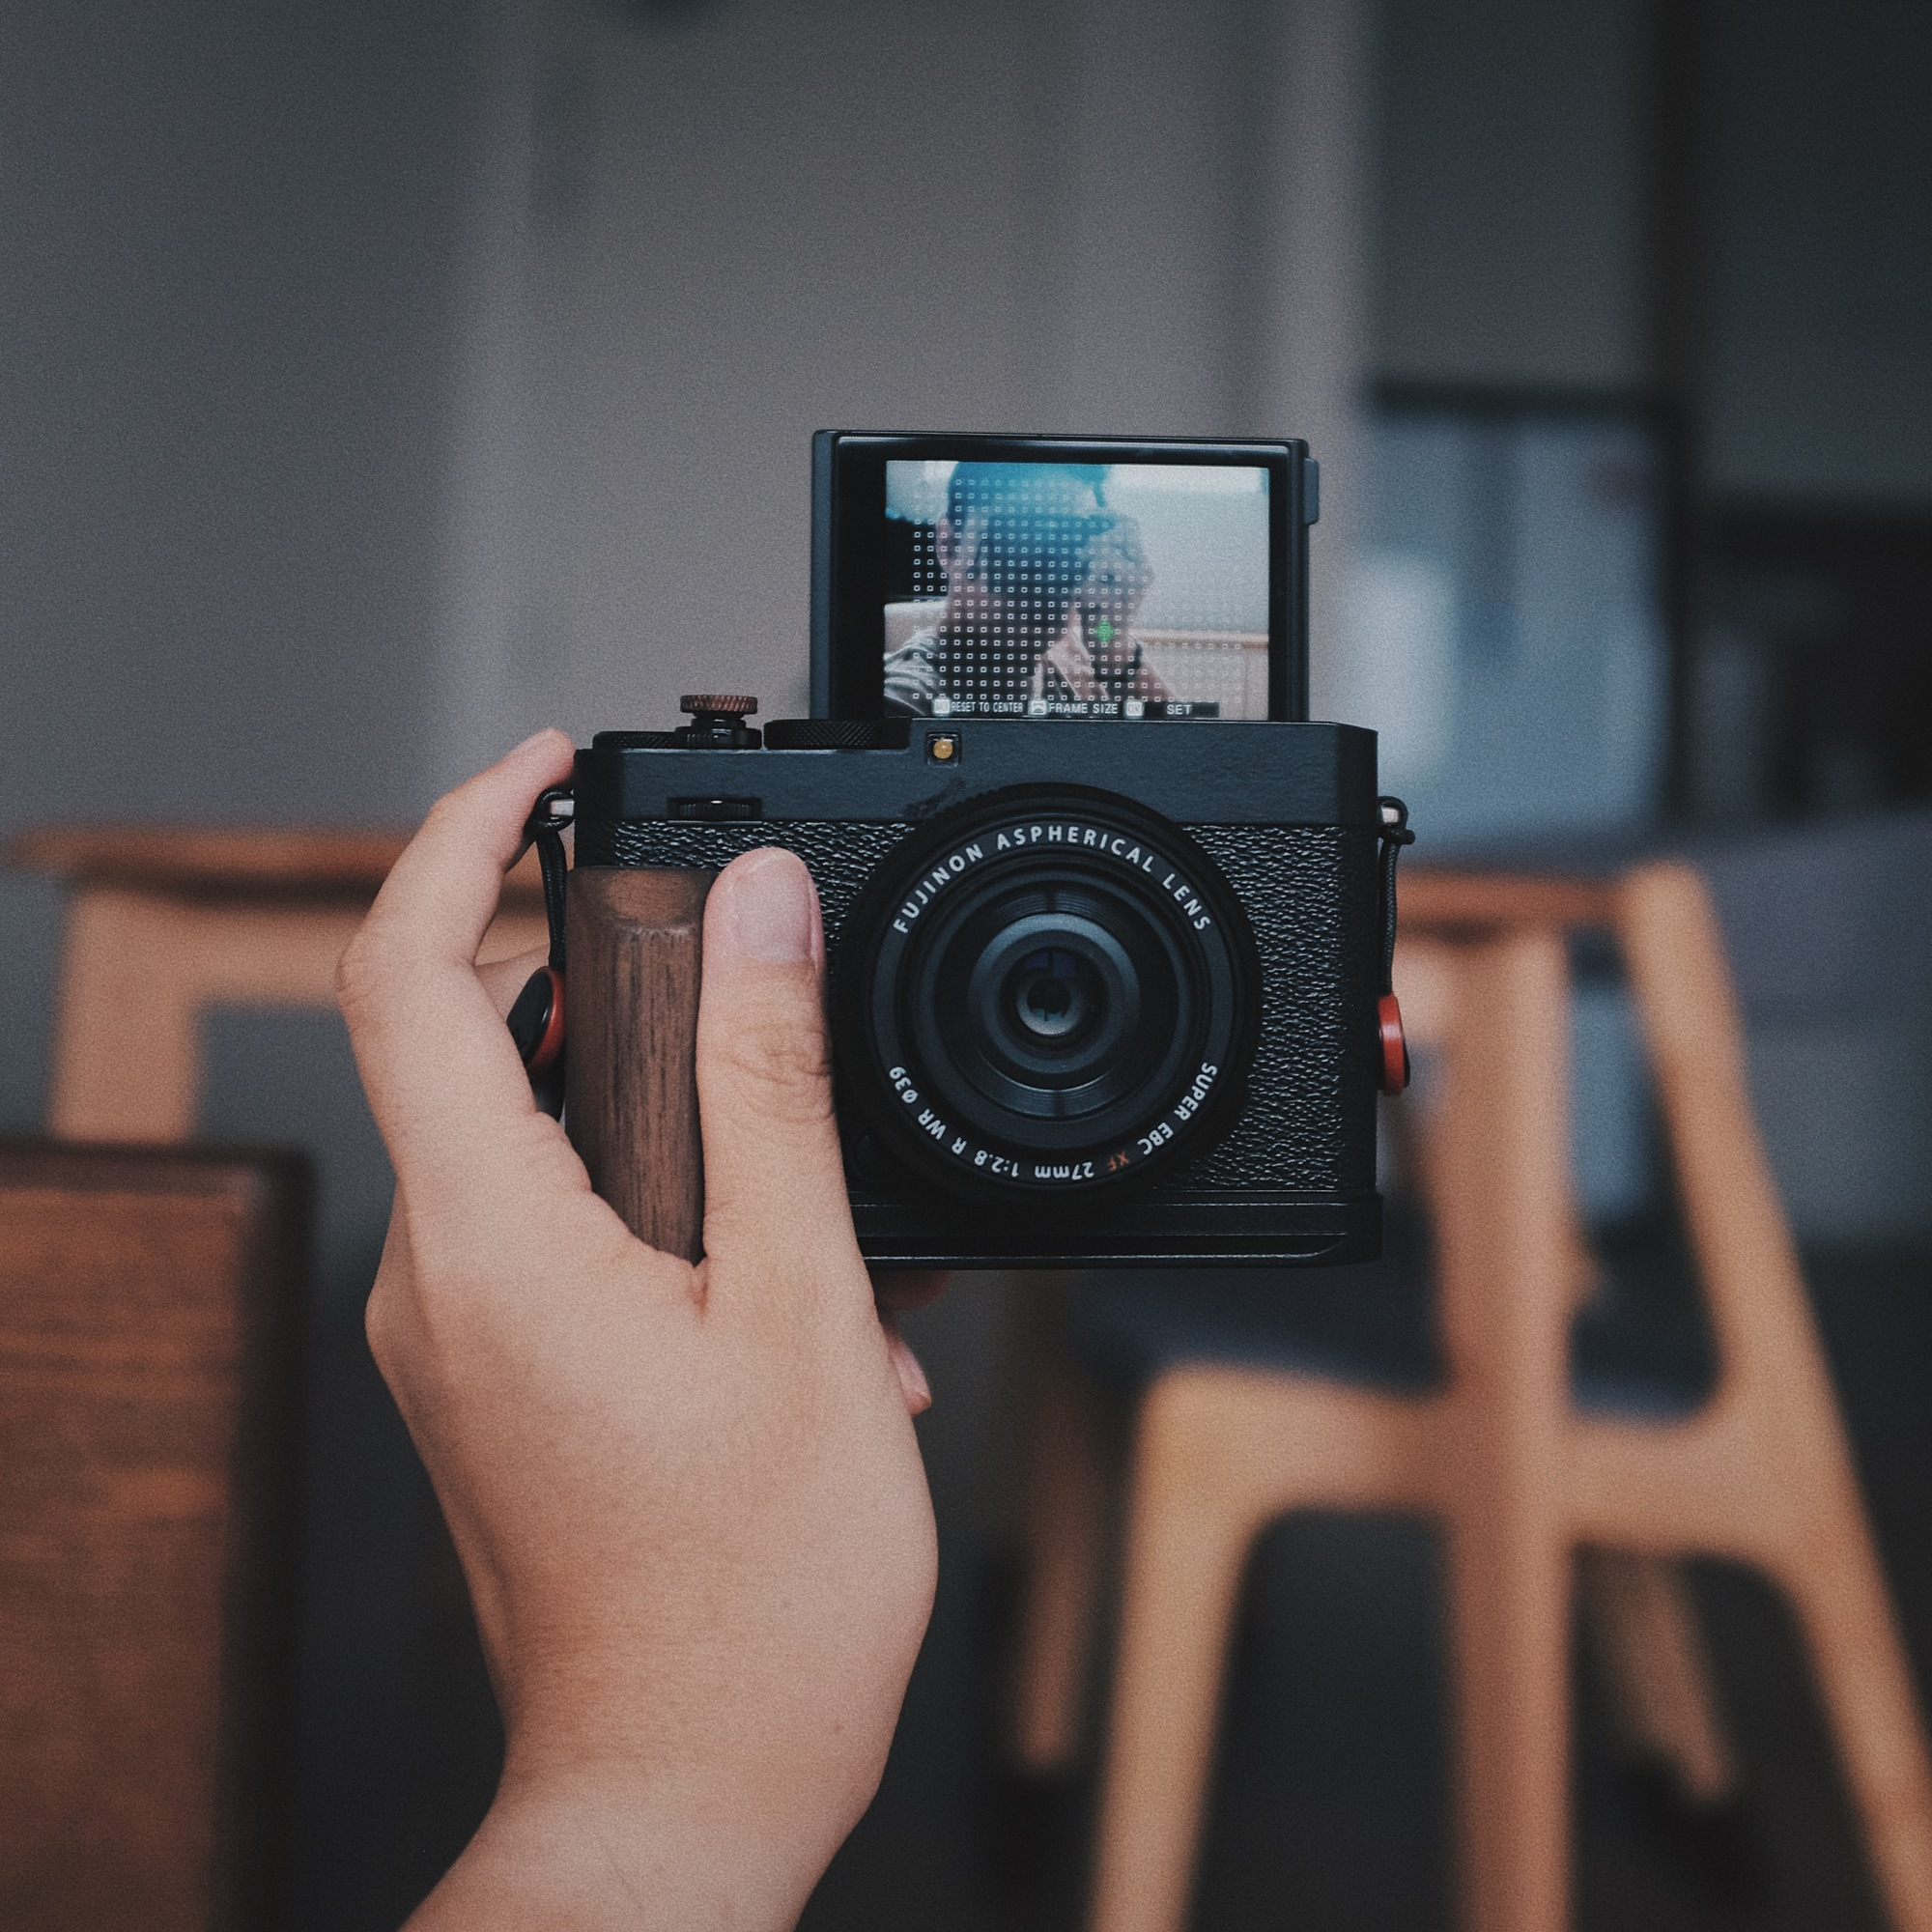
\includegraphics[width=\linewidth]{\envfinaldir/coverpic-prod.jpg}\par
            % \vskip 30pt
            \vfill

            \normalsize\rmfamily\scshape
            \copyright{} The Web Digest Project \hfill\large \envdatestr
        \end{center}
    \end{titlepage}
    % \restoregeometry
}
\newcommand{\simplehref}[1]{%
    \textcolor{blue!80!green}{\href{#1}{#1}}%
}
\renewcommand{\contentsname}{\center\Huge\sffamily\bfseries Contents\par\vskip 20pt}
\newcounter{ipartcounter}
\setcounter{ipartcounter}{0}
\newcommand{\ipart}[1]{
    % \vskip 20pt
    \clearpage
    \stepcounter{ipartcounter}
    \phantomsection
    \addcontentsline{toc}{chapter}{#1}
    % \begin{center}
    %     \Huge
    %     \sffamily\bfseries
    %     #1
    % \end{center}
    % \vskip 20pt plus 7pt
}
\newcounter{ichaptercounter}
\setcounter{ichaptercounter}{0}
\newcommand{\ichapter}[1]{
    % \vskip 20pt
    \clearpage
    \stepcounter{ichaptercounter}
    \phantomsection
    \addcontentsline{toc}{section}{\numberline{\arabic{ichaptercounter}}#1}
    \begin{center}
        \Huge
        \sffamily\bfseries
        #1
    \end{center}
    \vskip 20pt plus 7pt
}
\newcommand{\entrytitlefont}[1]{\subsection*{\raggedright\Large\sffamily\bfseries#1}}
\newcommand{\entryitemGeneric}[2]{
    % argv: title, url
    \parbox{\linewidth}{
        \entrytitlefont{#1}\par\vskip 5pt
        \footnotesize\ttfamily\mdseries
        \simplehref{#2}
    }\vskip 11pt plus 11pt minus 1pt
}
\newcommand{\entryitemGithub}[3]{
    % argv: title, url, desc
    \parbox{\linewidth}{
        \entrytitlefont{#1}\par\vskip 5pt
        \footnotesize\ttfamily\mdseries
        \simplehref{#2}\par\vskip 5pt
        \small\rmfamily\mdseries#3
    }\vskip 11pt plus 11pt minus 1pt
}
\newcommand{\entryitemAp}[3]{
    % argv: title, url, desc
    \parbox{\linewidth}{
        \entrytitlefont{#1}\par\vskip 5pt
        \footnotesize\ttfamily\mdseries
        \simplehref{#2}\par\vskip 5pt
        \small\rmfamily\mdseries#3
    }\vskip 11pt plus 11pt minus 1pt
}
\newcommand{\entryitemHackernews}[3]{
    % argv: title, hnurl, rawurl
    % \parbox{\linewidth}{
    %     \entrytitlefont{#1}\par\vskip 5pt
    %     \footnotesize\ttfamily\mdseries
    %     \simplehref{#3}\par
    %     \textcolor{black!50}{\href{#2}{#2}}
    % }\vskip 11pt plus 11pt minus 1pt
    \begin{minipage}{\linewidth}
            \entrytitlefont{#1}\par\vskip 5pt
            \footnotesize\ttfamily\mdseries
            \simplehref{#3}\par
            \textcolor{black!50}{\href{#2}{#2}}
    \end{minipage}\par\vskip 11pt plus 11pt minus 1pt
}







\begin{document}

\makeheader

\tableofcontents\clearpage




\ipart{Developers}
\ichapter{Hacker News}
\entryitemTwoLinks{Figma Files Registration Statement for Proposed Initial Public Offering}{https://news.ycombinator.com/item?id=44437316}{https://www.figma.com/blog/s1-public/}

\entryitemTwoLinks{Code⇄GUI bidirectional editing via LSP}{https://news.ycombinator.com/item?id=44435716}{https://jamesbvaughan.com/bidirectional-editing/}

\entryitemTwoLinks{The Fed says this is a cube of \$1M. They're off by half a million}{https://news.ycombinator.com/item?id=44435484}{https://calvin.sh/blog/fed-lie/}

\entryitemTwoLinks{PlanetScale for Postgres}{https://news.ycombinator.com/item?id=44434667}{https://planetscale.com/blog/planetscale-for-postgres}

\entryitemTwoLinks{Ask HN: Who is hiring? (July 2025)}{https://news.ycombinator.com/item?id=44434576}{https://news.ycombinator.com/item?id=44434576}

\entryitemTwoLinks{Feasibility study of a mission to Sedna - Nuclear propulsion and solar sailing}{https://news.ycombinator.com/item?id=44434062}{https://arxiv.org/abs/2506.17732}

\entryitemTwoLinks{Grammarly acquires Superhuman}{https://news.ycombinator.com/item?id=44433994}{https://www.reuters.com/business/grammarly-acquires-email-startup-superhuman-ai-platform-push-2025-07-01/}

\entryitemTwoLinks{Show HN: Spegel, a Terminal Browser That Uses LLMs to Rewrite Webpages}{https://news.ycombinator.com/item?id=44433409}{https://simedw.com/2025/06/23/introducing-spegel/}

\entryitemTwoLinks{Show HN: Jobs by Referral: Find jobs in your LinkedIn network}{https://news.ycombinator.com/item?id=44433386}{https://jobsbyreferral.com/}

\entryitemTwoLinks{Scientists identify culprit behind biggest-ever U.S. honey bee die-off}{https://news.ycombinator.com/item?id=44432467}{https://www.science.org/content/article/scientists-identify-culprit-behind-biggest-ever-u-s-honeybee-die}

\entryitemTwoLinks{Cloudflare to introduce pay-per-crawl for AI bots}{https://news.ycombinator.com/item?id=44432385}{https://blog.cloudflare.com/introducing-pay-per-crawl/}

\entryitemTwoLinks{OpenFLOW – Quickly make beautiful infrastructure diagrams local to your machine}{https://news.ycombinator.com/item?id=44431178}{https://github.com/stan-smith/OpenFLOW}

\entryitemTwoLinks{Aging-related inflammation is not universal across human populations}{https://news.ycombinator.com/item?id=44430984}{https://www.publichealth.columbia.edu/news/aging-related-inflammation-not-universal-across-human-populations}

\entryitemTwoLinks{Small language models are the future of agentic AI}{https://news.ycombinator.com/item?id=44430311}{https://arxiv.org/abs/2506.02153}

\entryitemTwoLinks{Why email startups fail}{https://news.ycombinator.com/item?id=44429457}{https://forwardemail.net/en/blog/docs/email-startup-graveyard-why-80-percent-email-companies-fail}

\entryitemTwoLinks{Claude Code now supports hooks}{https://news.ycombinator.com/item?id=44429225}{https://docs.anthropic.com/en/docs/claude-code/hooks}

\entryitemTwoLinks{Melbourne man discovers extensive model train network underneath house}{https://news.ycombinator.com/item?id=44429182}{https://www.sbs.com.au/news/article/i-was-shocked-melbourne-mans-unbelievable-find-after-buying-house/m4sksfer8}

\entryitemTwoLinks{Show HN: A continuation of IRS Direct File that can be self-hosted}{https://news.ycombinator.com/item?id=44428438}{https://github.com/openfiletax/openfile}

\entryitemTwoLinks{The new skill in AI is not prompting, it's context engineering}{https://news.ycombinator.com/item?id=44427757}{https://www.philschmid.de/context-engineering}

\entryitemTwoLinks{Price of rice in Japan falls below ¥4k per 5kg}{https://news.ycombinator.com/item?id=44427147}{https://www.japantimes.co.jp/news/2025/06/24/japan/japan-rice-price-falls-below-4000/}


\ipart{Developers~~~~(zh-Hans)}
\ichapter{Solidot}
\entryitemGeneric{\hskip 0pt{}Cloudflar 测试对 AI 机器人抓取内容收费}{https://www.solidot.org/story?sid=81697}

\entryitemGeneric{\hskip 0pt{}Sci-Hub 探索模因币的资助模式}{https://www.solidot.org/story?sid=81696}

\entryitemGeneric{\hskip 0pt{}Steam 推出新的游戏性能监视器}{https://www.solidot.org/story?sid=81695}

\entryitemGeneric{\hskip 0pt{}Windows 11 25H2 与 24H2 区别不大}{https://www.solidot.org/story?sid=81694}

\entryitemGeneric{\hskip 0pt{}Android 未来可能会警告用户手机连接了假基站}{https://www.solidot.org/story?sid=81693}

\entryitemGeneric{\hskip 0pt{}发表在 arXiv 上的论文被发现隐含 AI 指令}{https://www.solidot.org/story?sid=81692}

\entryitemGeneric{\hskip 0pt{}苹果考虑用 Anthropic 或 OpenAI 的模型驱动新版本的 Siri  }{https://www.solidot.org/story?sid=81691}

\entryitemGeneric{\hskip 0pt{}微软 Windows 操作系统三年流失了 4 亿用户}{https://www.solidot.org/story?sid=81690}

\entryitemGeneric{\hskip 0pt{}Tumblr 搁置后端迁移到 WordPress 和联邦宇宙整合的计划}{https://www.solidot.org/story?sid=81689}

\entryitemGeneric{\hskip 0pt{}Google 购买了 200MW 还不存在的聚变能源}{https://www.solidot.org/story?sid=81688}

\entryitemGeneric{\hskip 0pt{}中国的纸币和硬币在快速消失}{https://www.solidot.org/story?sid=81687}

\entryitemGeneric{\hskip 0pt{}服务器 GPU 配备太多的显存会导致 Linux 系统休眠出现问题}{https://www.solidot.org/story?sid=81686}

\entryitemGeneric{\hskip 0pt{}Fedora 44 不会停止支持 32 位}{https://www.solidot.org/story?sid=81685}

\entryitemGeneric{\hskip 0pt{}科学家在量子尺度验证守恒定律}{https://www.solidot.org/story?sid=81684}

\entryitemGeneric{\hskip 0pt{}比特币钱包地址暴露黑客 IntelBroker 的英籍身份}{https://www.solidot.org/story?sid=81683}

\entryitemGeneric{\hskip 0pt{}对 AI 的反对之声逐渐高涨}{https://www.solidot.org/story?sid=81682}

\entryitemGeneric{\hskip 0pt{}NSA 鼓励使用内存安全语言}{https://www.solidot.org/story?sid=81681}

\entryitemGeneric{\hskip 0pt{}小行星 2024 YR4 撞击月球概率上升至 1/25}{https://www.solidot.org/story?sid=81679}

\entryitemGeneric{\hskip 0pt{}碳记录显示人类五万年前开始大规模用火}{https://www.solidot.org/story?sid=81678}

\entryitemGeneric{\hskip 0pt{}研究发现消费者对 AI 产品信任度低}{https://www.solidot.org/story?sid=81677}\ichapter{V2EX}
\entryitemGeneric{\hskip 0pt{}[小米] 去看了小米 YU7 了,感觉有点失望}{https://www.v2ex.com/t/1142380}

\entryitemGeneric{\hskip 0pt{}[生活] 咨询一下各位佬,孩子出生你们是怎么带的?}{https://www.v2ex.com/t/1142379}

\entryitemGeneric{\hskip 0pt{}[优惠信息] 免费兑换任意 JetBrains 3 个月高级版}{https://www.v2ex.com/t/1142378}

\entryitemGeneric{\hskip 0pt{}[问与答] 怎么我打开首页出现广告了, v2 终于变质了?}{https://www.v2ex.com/t/1142377}

\entryitemGeneric{\hskip 0pt{}[问与答] 昨天领的 jetbrain all products,到期后还能永久使用当前的这个版本吗?}{https://www.v2ex.com/t/1142376}

\entryitemGeneric{\hskip 0pt{}[问与答] larix broadcaster 收费了有没有类似软件免费或者便宜一点的支持竖屏的 安卓手机推流 rtmp}{https://www.v2ex.com/t/1142375}

\entryitemGeneric{\hskip 0pt{}[分享发现] 金融计算器}{https://www.v2ex.com/t/1142374}

\entryitemGeneric{\hskip 0pt{}[远程工作] 招聘远程全职 IOS(续有安卓开发经验), 3500 美金/月}{https://www.v2ex.com/t/1142373}

\entryitemGeneric{\hskip 0pt{}[问与答] 求推荐一款主板,挑主板好繁琐啊,有些主板在官网上都没有写支持 Linux 。}{https://www.v2ex.com/t/1142372}

\entryitemGeneric{\hskip 0pt{}[推广] 活钱 12 | 月光族福音! 3 个简单存钱法}{https://www.v2ex.com/t/1142369}

\entryitemGeneric{\hskip 0pt{}[问与答] 狗血剧情就出现在我身边!}{https://www.v2ex.com/t/1142368}

\entryitemGeneric{\hskip 0pt{}[随想] 不得不感叹一下商人的脑子真好使 - 在 20250701 出现 Jetbrains 一年免费兑换码之后出现的商品}{https://www.v2ex.com/t/1142367}

\entryitemGeneric{\hskip 0pt{}[Vue.js] 开发一款轻便简洁的论坛程序}{https://www.v2ex.com/t/1142366}

\entryitemGeneric{\hskip 0pt{}[分享发现] 深夜推荐蟑螂药,效果太好了强烈推荐}{https://www.v2ex.com/t/1142365}

\entryitemGeneric{\hskip 0pt{}[问与答] 安卓微软 auth 的二验怎么在 ios 设备上也整一份?}{https://www.v2ex.com/t/1142364}

\entryitemGeneric{\hskip 0pt{}[宽带症候群] 精品网是被故意搞坏了?}{https://www.v2ex.com/t/1142362}

\entryitemGeneric{\hskip 0pt{}[分享创造] 学习运维咖啡老哥也搞了个拼图网站,欢迎使用}{https://www.v2ex.com/t/1142361}

\entryitemGeneric{\hskip 0pt{}[分享发现] 分享一个刚上线的领带打结教程网站}{https://www.v2ex.com/t/1142360}

\entryitemGeneric{\hskip 0pt{}[生活] 开源节流计划}{https://www.v2ex.com/t/1142359}

\entryitemGeneric{\hskip 0pt{}[程序员] DeepSeek 每次都是英文回答,如何避免}{https://www.v2ex.com/t/1142358}

\entryitemGeneric{\hskip 0pt{}[NAS] Nas 设备求推荐}{https://www.v2ex.com/t/1142357}

\entryitemGeneric{\hskip 0pt{}[求职] 西安有机会吗 嵌入式}{https://www.v2ex.com/t/1142356}

\entryitemGeneric{\hskip 0pt{}[Apple] macos 被玩坏了,进不去,求指点}{https://www.v2ex.com/t/1142355}

\entryitemGeneric{\hskip 0pt{}[宽带症候群] 服务器被 20.171.207.0/24 刷流量}{https://www.v2ex.com/t/1142353}

\entryitemGeneric{\hskip 0pt{}[程序员] 古早数字生活方式梦核}{https://www.v2ex.com/t/1142352}

\entryitemGeneric{\hskip 0pt{}[生活] 干快递半年了,大伙儿有什么想问的}{https://www.v2ex.com/t/1142350}

\entryitemGeneric{\hskip 0pt{}[程序员] sagesai: 10 倍提升 devops 效率}{https://www.v2ex.com/t/1142348}

\entryitemGeneric{\hskip 0pt{}[问与答] 有比较靠谱和高性价比的发卡站点推荐吗?}{https://www.v2ex.com/t/1142347}

\entryitemGeneric{\hskip 0pt{}[问与答] 抛弃苹果以后 airplay 音响咋办?}{https://www.v2ex.com/t/1142346}

\entryitemGeneric{\hskip 0pt{}[生活] 分享两个生活经验}{https://www.v2ex.com/t/1142345}

\entryitemGeneric{\hskip 0pt{}[Apple] [微信 For Mac] 4.X 版本已经上架商店了}{https://www.v2ex.com/t/1142344}

\entryitemGeneric{\hskip 0pt{}[酷工作] [深圳] 招聘 运维工程师}{https://www.v2ex.com/t/1142340}

\entryitemGeneric{\hskip 0pt{}[阅读] 同志们,杂志常用双栏排版,在 15.6 寸显示器上根本不方便看,你们怎么解决的?}{https://www.v2ex.com/t/1142339}

\entryitemGeneric{\hskip 0pt{}[分享发现] 原来谷歌的人机验证只要做对最后一个就可以}{https://www.v2ex.com/t/1142338}

\entryitemGeneric{\hskip 0pt{}[教育] 求高考志愿指导}{https://www.v2ex.com/t/1142337}

\entryitemGeneric{\hskip 0pt{}[分享发现] 现在的 v2 变味了}{https://www.v2ex.com/t/1142336}

\entryitemGeneric{\hskip 0pt{}[分享创造] iPad 、 iPhone 版本也上线了,再送一批兑换码,用 Safari 的可以看过来}{https://www.v2ex.com/t/1142335}

\entryitemGeneric{\hskip 0pt{}[问与答] 推荐一个运动手环}{https://www.v2ex.com/t/1142334}

\entryitemGeneric{\hskip 0pt{}[生活] 吐个槽,现在在自行车锁怎么越用越失望。}{https://www.v2ex.com/t/1142333}

\entryitemGeneric{\hskip 0pt{}[分享发现] 免费 JetBrains 后续:系会议码,新领取需提交参会证明}{https://www.v2ex.com/t/1142332}

\entryitemGeneric{\hskip 0pt{}[酷工作] 字节-番茄小说-招前端实习生-面向 2026 年毕业生(社招也有}{https://www.v2ex.com/t/1142331}

\entryitemGeneric{\hskip 0pt{}[生活] 我被中医治好过的症状:慢性支气管炎/心脑不适/干眼症}{https://www.v2ex.com/t/1142330}

\entryitemGeneric{\hskip 0pt{}[问与答] 观抖音`` Python 帮''话术有感}{https://www.v2ex.com/t/1142329}

\entryitemGeneric{\hskip 0pt{}[Terminal] MacOS 上的 SSH 工具除了 Termius 有其他替换吗?}{https://www.v2ex.com/t/1142326}

\entryitemGeneric{\hskip 0pt{}[分享发现] EdgeOne 国际版用上了,来测下速吧}{https://www.v2ex.com/t/1142325}

\entryitemGeneric{\hskip 0pt{}[问与答] coze 上的工作流都不能导入导出的吗?}{https://www.v2ex.com/t/1142324}

\entryitemGeneric{\hskip 0pt{}[问与答] 设计类网课资源去哪找呢}{https://www.v2ex.com/t/1142323}

\entryitemGeneric{\hskip 0pt{}[Cursor] 可能迄今为止最好的 Cursor RULE. 有状态、DDD(Document Driven Development)}{https://www.v2ex.com/t/1142322}

\entryitemGeneric{\hskip 0pt{}[JetBrains] 续订全家桶时找不到 renew 按钮}{https://www.v2ex.com/t/1142321}

\entryitemGeneric{\hskip 0pt{}[职场话题] 小调查: 28 岁程序员,上海、杭州,(已)离开/(打算)定居?}{https://www.v2ex.com/t/1142320}


\ipart{Generic News}







\clearpage
\leavevmode\vfill
\footnotesize

Copyright \copyright{} 2023-2025 Neruthes and other contributors.

This document is published with CC BY-NC-ND 4.0 license.

The entries listed in this newsletter may be copyrighted by their respective creators.

This newsletter is generated by the Web Digest project.

The newsletters are also delivered via Telegram channel \CJKunderline{\href{https://t.me/webdigestchannel}{https://t.me/webdigestchannel}}.\\
RSS feed is available at \CJKunderline{\href{https://webdigest.pages.dev/rss.xml}{https://webdigest.pages.dev/rss.xml}}.

This newsletter is available in PDF at
\CJKunderline{\href{https://webdigest.pages.dev/}{https://webdigest.pages.dev/}}.

The source code being used to generate this newsletter is available at\\
\CJKunderline{\href{https://github.com/neruthes/webdigest}{https://github.com/neruthes/webdigest}}.

This newsletter is also available in
\CJKunderline{\href{http://webdigest.pages.dev/readhtml/\envyear/WebDigest-20250702.html}{HTML}} and
\CJKunderline{\href{https://github.com/neruthes/webdigest/blob/master/markdown/\envyear/WebDigest-20250702.md}{Markdown}}.


\coverpic{https://unsplash.com/photos/aerial-view-of-a-densely-populated-city-with-highways-LzLyam-1B5E}{ZHENYU LUO}


\end{document}
